\documentclass[
	8pt, % Set the default font size, options include: 8pt, 9pt, 10pt, 11pt, 12pt, 14pt, 17pt, 20pt
	%t, % Uncomment to vertically align all slide content to the top of the slide, rather than the default centered
	%aspectratio=169, % Uncomment to set the aspect ratio to a 16:9 ratio which matches the aspect ratio of 1080p and 4K screens and projectors
]{beamer}
\graphicspath{{Images/}{./}}
\usepackage{booktabs} 
\usetheme{Madrid}
\usecolortheme{seahorse}
\usefonttheme{default} 
\usepackage{palatino}
\usepackage[default]{opensans}
\useinnertheme{circles}

\title[Sustainable Bonds]{Sustainable Bond Metrics} 
\subtitle{IT Skills for Research} 
\author[Patrick Röthlisberger \and Stefan Aeby]{Patrick Röthlisberger \and Stefan Aeby} % Presenter name(s), the optional parameter can contain a shortened version to appear on the bottom of every slide, while the main parameter will appear on the title slide

\institute[UC]{University of Zürich \\ \smallskip \textit{roer@zhaw.ch} \textit{aebystefan@gmail.com}} 
\date[\today]{\\ \today} % 
\begin{document}

%	TITLE SLIDE

\begin{frame}
	\titlepage % Output the title slide, automatically created using the text entered in the PRESENTATION INFORMATION block above
\end{frame}

%	TABLE OF CONTENTS SLIDE

% The table of contents outputs the sections and subsections that appear in your presentation, specified with the standard \section and \subsection commands. You may either display all sections and subsections on one slide with \tableofcontents, or display each section at a time on subsequent slides with \tableofcontents[pausesections]. The latter is useful if you want to step through each section and mention what you will discuss.

\begin{frame}
	\frametitle{Presentation Overview} 
	
	\tableofcontents
\end{frame}

%	PRESENTATION BODY SLIDES

\section{Database} 

\begin{frame}
	\frametitle{Database}
	
	Data initially comes from the \alert{Bloomberg} terminal. We created the following search conditions:
 \bigskip % Vertical whitespace
 \begin{enumerate}
    \item Bonds: All
    \item (and) BICS Classification: Exclude Sovereigns, or Government, Regional Government, Supranational, State Development Banks, Liquidation Agencies, or Central Banks, or Local Government.
    \item (and) Green Instrument - Indicator as Yes
    \item (or) Social Instrument - Indicator as Yes
    \item (or) Sustainability Linked Indicator as Yes
    \item (and) Emission Date later than 12/31/2014
    \item (and) Country/Region of Issuance including Europe
\end{enumerate}
\end{frame}

\begin{frame}{Data II}
 The data from Bloomberg includes an identifier. The identifier is then used to create additional columns with the financials of the issuers ultimate parent company. The following data is fetched via a Refinititv Eikon API in Excel:
 
 \begin{align}
    =RDP.Data(Identifier Cell Reference;"Code";"Sdate=\#1";;Date Cell Reference) 
 \end{align}
\end{frame}

\begin{frame}{Data III}
These are the captions used to fetch company data in Refinititv Eikon:
\begin{itemize}
    \item \textbf{Emission Date -1}
    \item \textbf{Total Assets}: \textit{TR.F.TotAssets} in Emission Date -1
    \item \textbf{Market Cap:} \textit{TR.CompanyMarketCapitalization} in Emission Date -1
    \item \textbf{Tobins Q: }Tot.Assets divided by CompanyMarketCapitalization
    \item \textbf{Leverage:} \textit{TR.PCLTDebtToTotEquPct} in Emission Date -1
    \item \textbf{Cash Flow to total Assets:} \textit{TR.F.NetCFOpToTotAssets} in Emission Date -1
    \item \textbf{Return on Asset (ROA):} \textit{TR.F.ReturnAvgTotAssetsPctTTM} in Emission Date -1
    \item \textbf{Return on Equity (ROE):} \textit{TR.F.ReturnAvgComEqPctTTM} in Emission Date -1
    \item \textbf{TRBC Economic Sector:} \textit{TR.TRBCEconomicSector} of Parent
\end{itemize}
    
\end{frame}
\section{Market}
\begin{frame}{Market Overview}
    \begin{figure}[H]
    \centering
    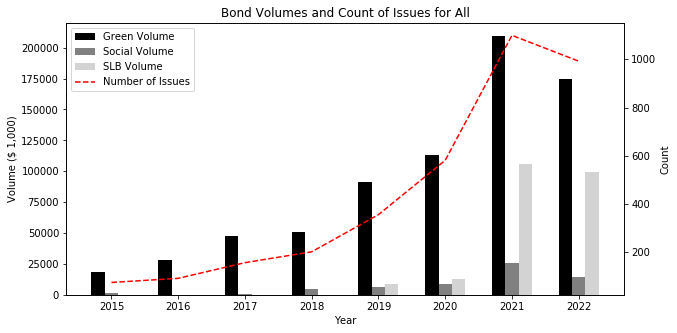
\includegraphics[width=0.85\linewidth]{VolumeCount.png}
    \caption{Sustainable Bonds Emissions in Europe (Data from Bloomberg)}
\label{fig:market}
\end{figure}
\end{frame}
\section{Bond Metrics}
    \begin{frame}{Summary Tables I}
    Table \ref{table:2} gives a short overview on the numbers on Coupon (Kpn), Emission Volume (Ausg\_Mge) and Maturity while table \ref{table:1} is giving the number of outstanding bonds for each category:
        \begin{columns}[c]
            \begin{column}{0.4\textwidth}
                \begin{table}[htbp]
                \centering
                \begin{tabular}{ll}
                \toprule
                Green Instrument & 3301 \\
                Social Bond & 199 \\
                Sust Linked & 580 \\
                \bottomrule
                \end{tabular}
                \caption{Table with number of outstanding bonds}
                \label{table:1}
                \end{table}
                \end{column}
            \begin{column}{0.6\textwidth}
                \begin{table}[htbp]
                \centering
                \begin{tabular}{lll}
                \toprule
                {} & mean & std \\
                \midrule
                Ausg\_Mge & 300,412,618.30 & 348,381,822.82 \\
                Kpn & 2.67 & 2.49 \\
                Maturity & 7.43 & 16.68 \\
                \bottomrule
                \end{tabular}
                \caption{Table with summary statistics}
                \label{table:2}
                \end{table}
            \end{column}
    
    \end{columns}
\end{frame}

\begin{frame}{Summary Tables II}
 \begin{table}[h]
\centering
\begin{tabular}{lr}
\hline
Industry & Count \\
\hline
Financials & 351 \\
Utilities & 176 \\
Industrials & 109 \\
Real Estate & 101 \\
Basic Materials & 44 \\
Consumer Cyclicals & 44 \\
Technology & 25 \\
Consumer Non-Cyclicals & 23 \\
Energy & 16 \\
Healthcare & 10 \\
\hline
\end{tabular}
\caption{Industry Counts}
\label{table:3}
\end{table}
 
  %Enter other tables on industry and number of issuers  
\end{frame}

\begin{frame}{Summary Tables III}
 \begin{table}[h]
\centering
\caption{Green Instrument Statistics}
\begin{tabular}{lrrrrr}
\hline
 & TobinsQ & LTLeverage & CFtoAsset & ROA & ROE \\
\hline
count & 723.00 & 723.00 & 723.00 & 723.00 & 723.00 \\
mean & 0.39 & 147.48 & 0.03 & 2.46 & 9.53 \\
std & 0.99 & 129.69 & 0.04 & 3.43 & 9.93 \\
min & 0.00 & 0.00 & -0.07 & -9.20 & -34.39 \\
25\% & 0.05 & 71.50 & 0.01 & 0.45 & 5.49 \\
50\% & 0.22 & 117.21 & 0.03 & 1.32 & 8.86 \\
75\% & 0.41 & 158.68 & 0.06 & 3.11 & 12.02 \\
max & 16.82 & 1016.25 & 0.21 & 20.22 & 65.38 \\
\hline
\end{tabular}
\label{table:4}
\end{table}

\begin{table}[h]
\centering
\caption{Social Bond Statistics}
\begin{tabular}{lrrrrr}
\hline
 & TobinsQ & LTLeverage & CFtoAsset & ROA & ROE \\
\hline
count & 37.00 & 37.00 & 37.00 & 37.00 & 37.00 \\
mean & 0.21 & 128.00 & 0.03 & 2.35 & 11.24 \\
std & 0.25 & 68.26 & 0.04 & 2.71 & 7.29 \\
min & 0.01 & 14.90 & -0.02 & 0.03 & -1.23 \\
25\% & 0.03 & 91.99 & -0.00 & 0.39 & 6.36 \\
50\% & 0.06 & 120.99 & 0.02 & 0.70 & 9.02 \\
75\% & 0.34 & 138.39 & 0.05 & 5.62 & 15.21 \\
max & 0.95 & 382.56 & 0.14 & 9.75 & 32.97 \\
\hline
\end{tabular}
\label{table:5}
\end{table}
 
  %Enter other tables on industry and number of issuers  
\end{frame}

\begin{frame}{Summary Tables III}
  \begin{table}[h]
\centering
\caption{Sustainability Linked Statistics}
\begin{tabular}{lrrrrr}
\hline
 & TobinsQ & LTLeverage & CFtoAsset & ROA & ROE \\
\hline
count & 139.00 & 139.00 & 139.00 & 139.00 & 139.00 \\
mean & 3.31 & 100.37 & 0.07 & 2.53 & 7.27 \\
std & 20.24 & 56.29 & 0.04 & 4.82 & 15.60 \\
min & 0.03 & 0.10 & 0.00 & -12.19 & -48.28 \\
25\% & 0.33 & 61.69 & 0.05 & 1.75 & 5.76 \\
50\% & 0.48 & 112.65 & 0.07 & 2.16 & 8.60 \\
75\% & 0.63 & 117.00 & 0.08 & 4.14 & 11.97 \\
max & 169.55 & 375.29 & 0.32 & 21.60 & 81.53 \\
\hline
\end{tabular}
\label{table:6}
\end{table}  
\end{frame}

\begin{frame}{Graph Metrics}
%Splitt figures and make description
In the following slides, we present the most important insights in the analysis of the instruments. First
    \begin{figure}[H]
    \centering
    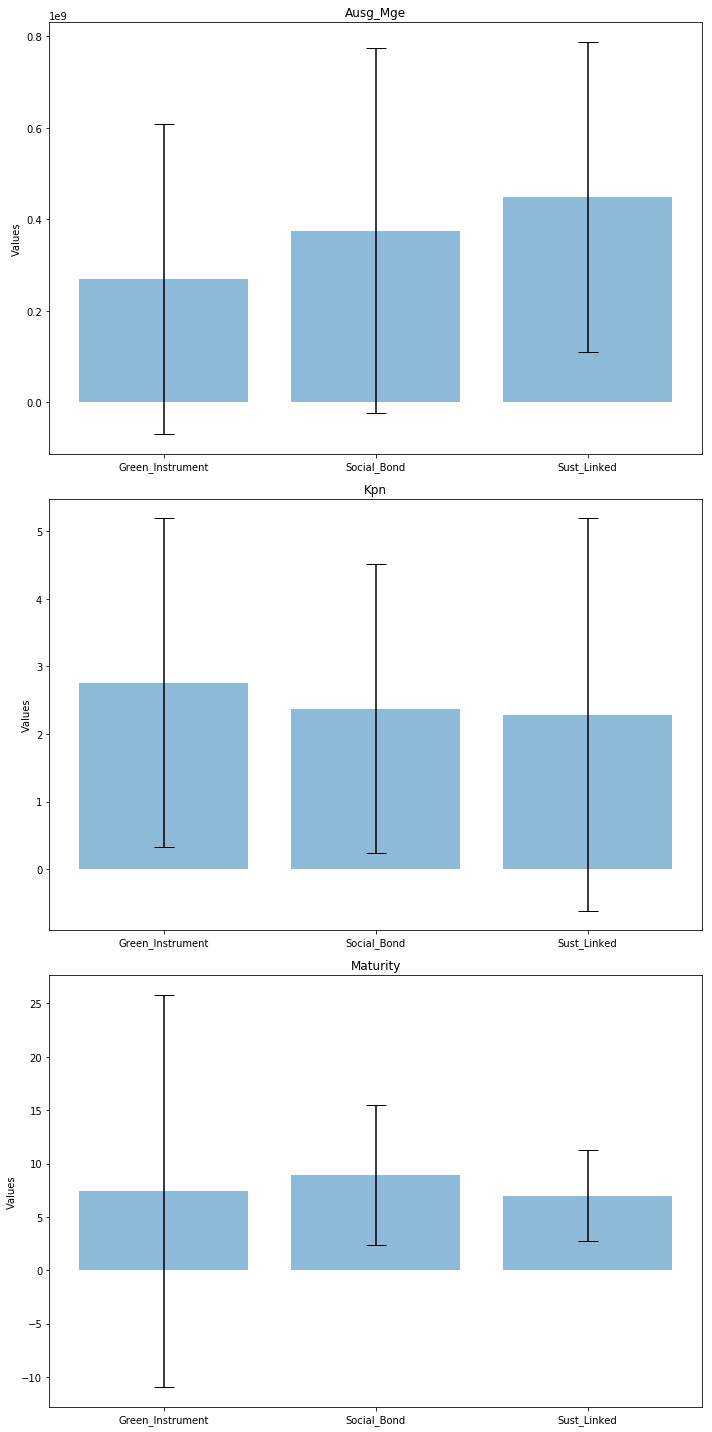
\includegraphics[width=0.8\linewidth, height=0.8\textheight, keepaspectratio]{Metrics_per_Bond.png}
    \caption{Coupon, Emission Volume and Maturity for each Bond Category}
\label{fig:Metrics}
\end{figure}
\end{frame}

\begin{frame}{Graph Metrics over Time}
    \begin{figure}[H]
    \centering
    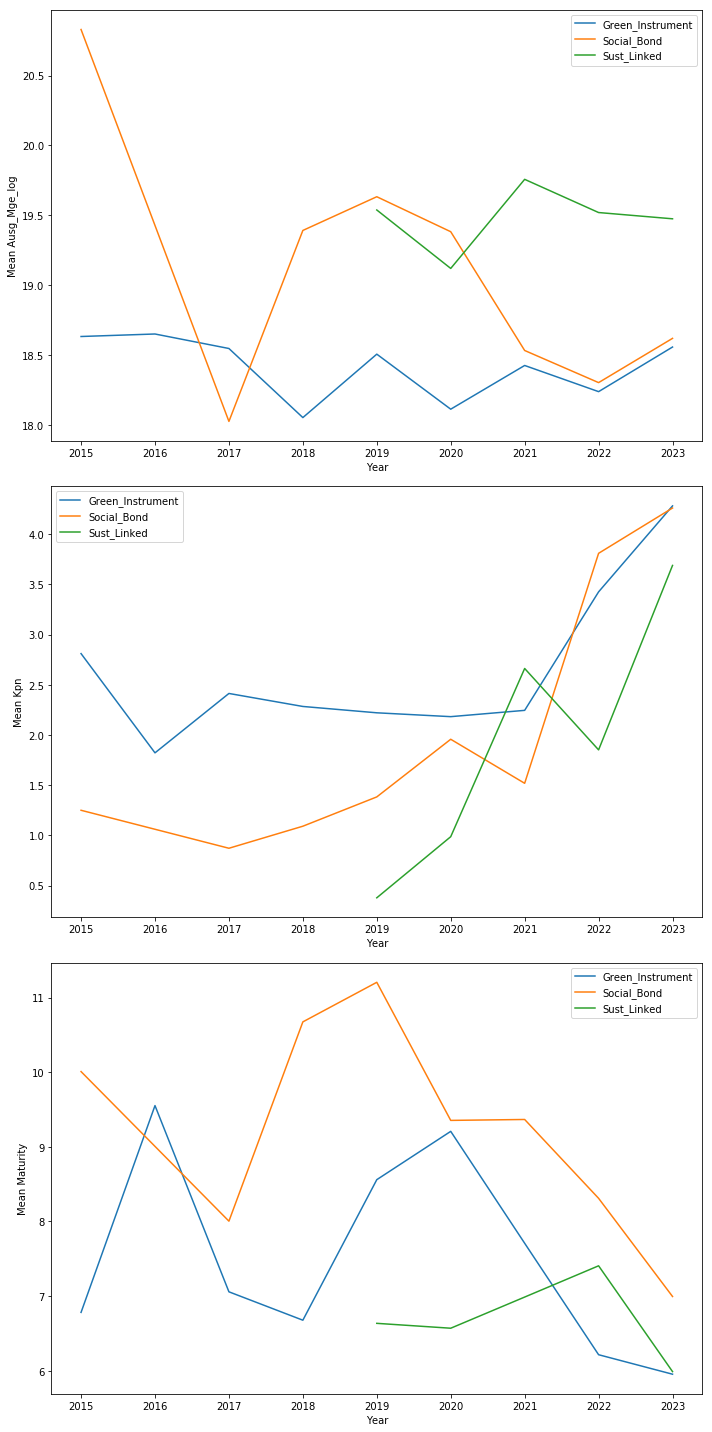
\includegraphics[width=0.8\linewidth, height=0.8\textheight, keepaspectratio]{Metrics_overtime.png}
    \caption{Coupon, Emission Volume and Maturity over time}
\label{fig:Metrics}
\end{figure}
\end{frame}

\begin{frame}{Graph Company Data}
    \begin{figure}[H]
    \centering
    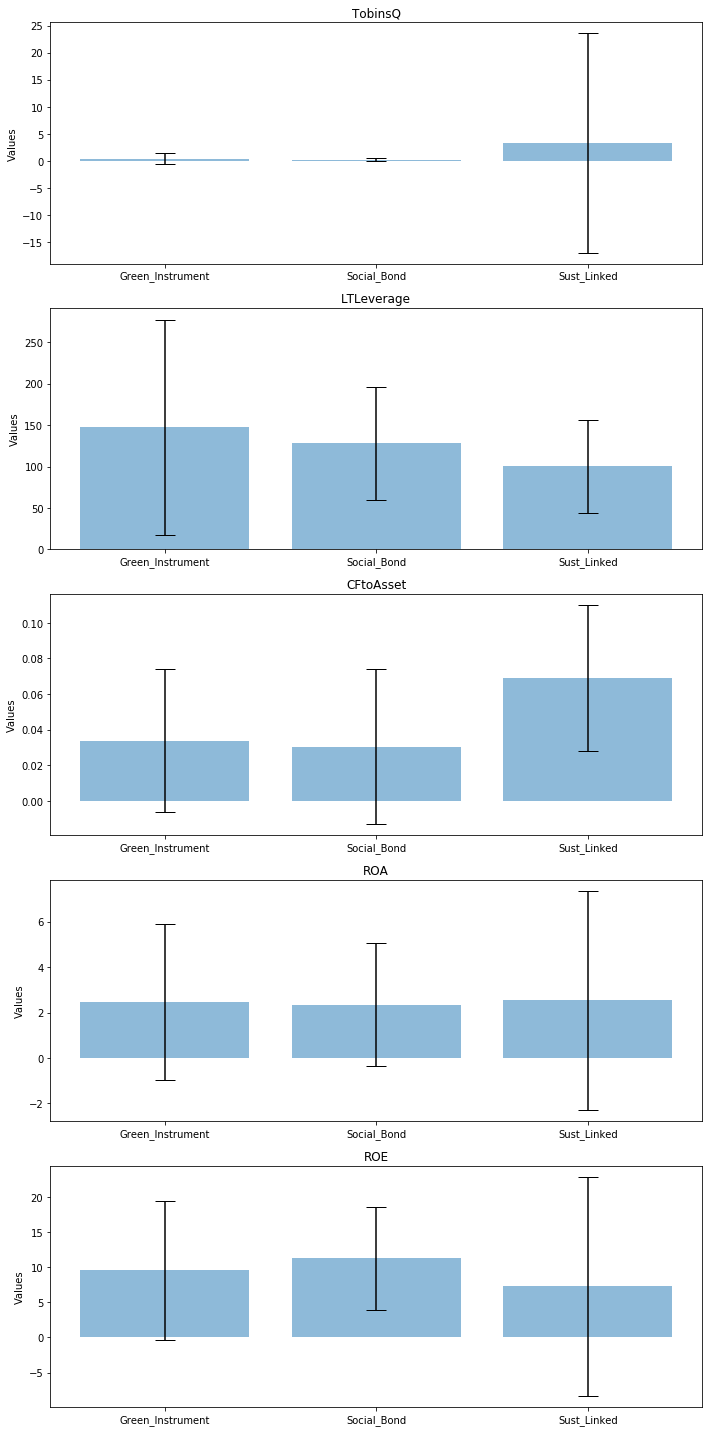
\includegraphics[width=0.8\linewidth, height=0.8\textheight, keepaspectratio]{Company_Data.png}
    \caption{Coupon, Emission Volume and Maturity over time}
\label{fig:Metrics}
\end{figure}
\end{frame}

\begin{frame}{Graph Company Data over Time}
    \begin{figure}[H]
    \centering
    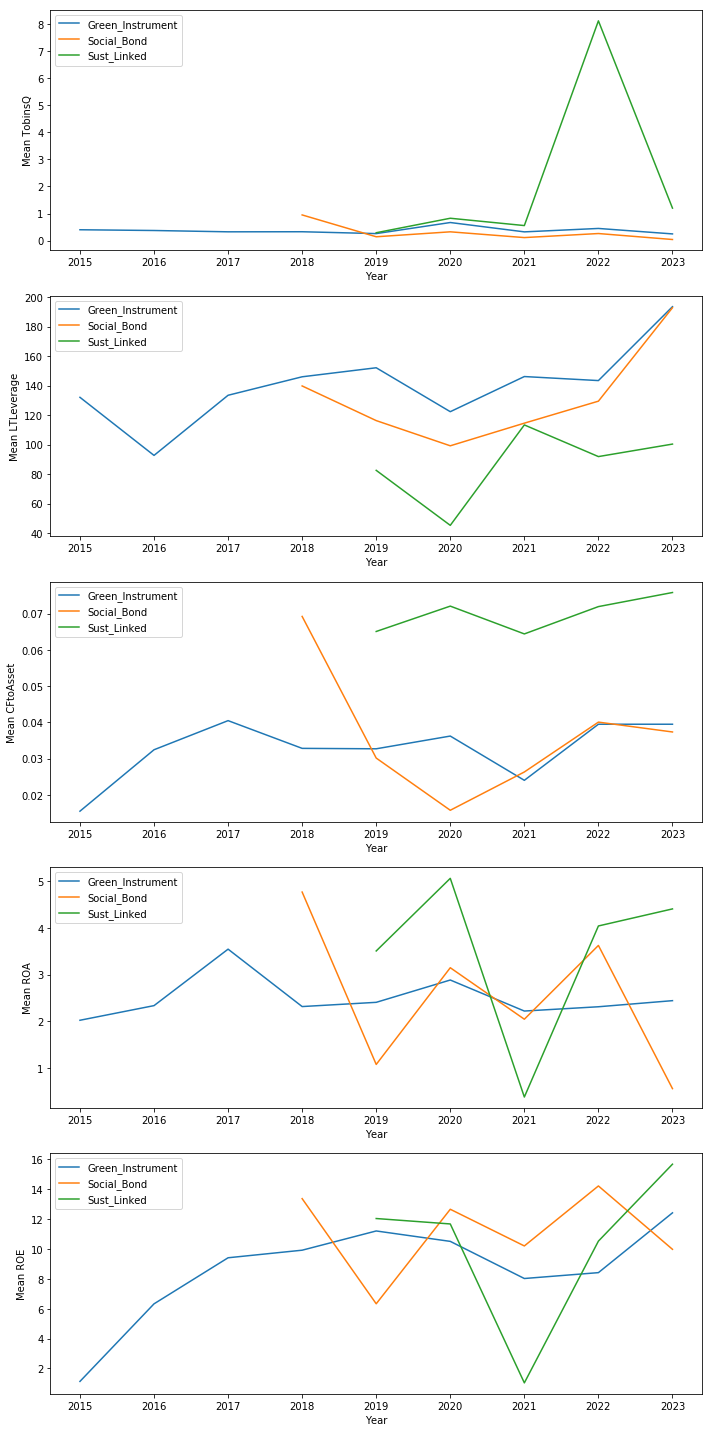
\includegraphics[width=0.8\linewidth, height=0.8\textheight, keepaspectratio]{Company_Data_overtime.png}
    \caption{Coupon, Emission Volume and Maturity over time}
\label{fig:Metrics}
\end{figure}
\end{frame}

\end{document} 